\let\negmpace\undefined
\let\negthickspace\undefined
\documentclass[journal]{IEEEtran}
\usepackage[a5paper, margin=10mm, onecolumn]{geometry}
%\usepackage{lmodern} % Ensure lmodern is loaded for pdflatex
\usepackage{tfrupee} % Include tfrupee package
\setlength{\headheight}{1cm} % Set the height of the header box
\setlength{\headsep}{0mm}     % Set the distance between the header box and the top of the text
\usepackage{xparse}
\usepackage{gvv-book}
\usepackage{gvv}
\usepackage{cite}
\usepackage{amsmath,amssymb,amsfonts,amsthm}
\usepackage{algorithmic}
\usepackage{graphicx}
\usepackage{textcomp}
\usepackage{xcolor}
\usepackage{txfonts}
\usepackage{listings}
\usepackage{enumitem}
\usepackage{mathtools}
\usepackage{gensymb}
\usepackage{comment}
\usepackage[breaklinks=true]{hyperref}
\usepackage{tkz-euclide} 
\usepackage{listings}
% \usepackage{gvv}                                        
\def\inputGnumericTable{}                                 
\usepackage[latin1]{inputenc}                                
\usepackage{color}                                            
\usepackage{array}                                            
\usepackage{longtable}                                       
\usepackage{calc}                                             
\usepackage{multirow}                                         
\usepackage{hhline}                                           
\usepackage{ifthen}                                           
\usepackage{lscape}
\renewcommand{\thefigure}{\theenumi}
\renewcommand{\thetable}{\theenumi}
\setlength{\intextsep}{10pt} % Space between text and floats
\numberwithin{equation}{enumi}
\numberwithin{figure}{enumi}
\renewcommand{\thetable}{\theenumi}
\begin{document}
\bibliographystyle{IEEEtran}
\title{4-4.2-6}
\author{EE24BTECH11030 - J.KEDARANANDA}
% \maketitle
% \newpage
% \bigskip
{\let\newpage\relax\maketitle}
\textbf{Question}:\\
Find the direction and normal vectors of the following line:\\
3x + 2 = 0
\\
\solution \\
\begin{table}[h!]
  \centering
  \begin{center}
    \begin{tabular}{|c|c|} 
        \hline
            \textbf{Variable} & \textbf{Value} \\ 
        \hline
            $\boldsymbol{BC}$ & 6 cm \\ 
        \hline
            $\boldsymbol{AB}$ & 5 cm \\ 
        \hline
            $\angle \vec{B}$  & $60^\circ$ \\
        \hline
    \end{tabular}
\end{center}  



  \caption{}
  \label{tabQuestion-4-4.2-6}
\end{table}\\
For the line of form Ax+By+C=0 the normal vector is given by
\begin{align}
    n&=\myvec{A\\B}\\
    A=3,B=0\\
    \implies n&=\myvec{3\\0}
\end{align}
Let the direction vector be d=$\myvec{a\\b}$
\begin{align}
    d^T.n&=0\\
    3a&=0\\
    \implies d&=\myvec{0\\-3}
\end{align}
\begin{figure}[h!]
    \centering
    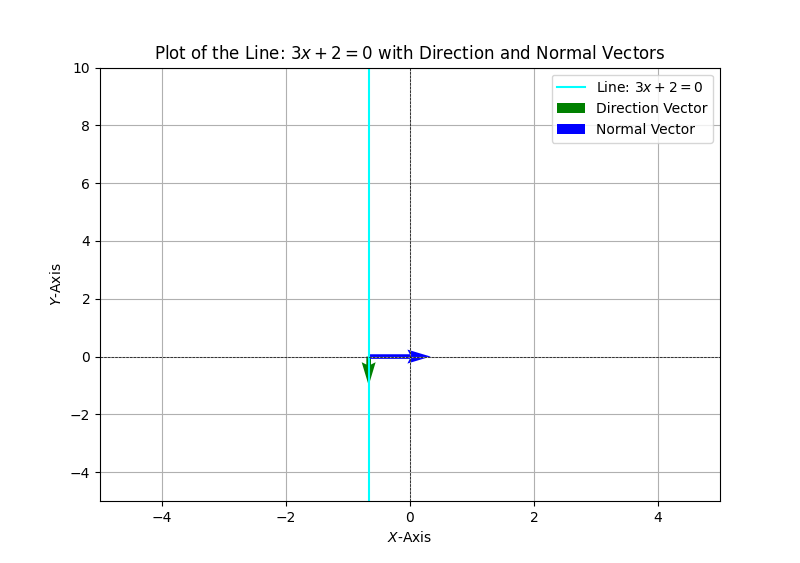
\includegraphics[width=\linewidth]{figs/fig1.png}
    \caption{ Line $Line 3x + 2 = 0$}
\end{figure}
\end{document}
